\documentclass[11pt]{article}
\usepackage{fullpage}
\usepackage{amsthm}
\usepackage{amsmath} \usepackage{amssymb}
\usepackage{graphicx}

\graphicspath{ {./imgs/} }

\setlength{\parindent}{0pt}

\title{Graphics (CO317)}
\author{Michael Tsang}

\newtheorem{defn}{Definition}
\newtheorem{eg}{Example}
\newtheorem{theo}{Theorem}
\newtheorem{lem}{Lemma}

\begin{document}

\maketitle

\section{Projections and Transformations}
\subsection{Device Independence}
Device dependent graphics primitive methods are:
\begin{verbatim}
  SetPixel(XCoord, YCoord, Colour);
  DrawLine(xs, ys, xf, yf);
\end{verbatim}

\textbf{Device independence} allows us to resize or transport a picture to a different operating system, and have it fit exactly in the window where we place it.
We define a \textbf{world coordinate system} when drawing objects, typically it will use a method of the kind:
\begin{verbatim}
  SetWindowCoords(Wxmin, Wymin, Wxmax, Wymax);
\end{verbatim}

The units of these arguments will depend on that application.
The application uses drawing primitives and these units to convert their numeric values to pixels, before the image is rendered on the screen.

In order to implement a world coordinate system, we need to be able to translate between world coordinates and the device or pixel coordinates.
We first find out the pixel coordinates of the window:
\begin{verbatim}
  GetWindowPixelCoords(Vxmin, Vymin, Vxmax, Vymax);
\end{verbatim}

\begin{figure}[h]
  \caption{World coordinate window against viewport on the screen.}
  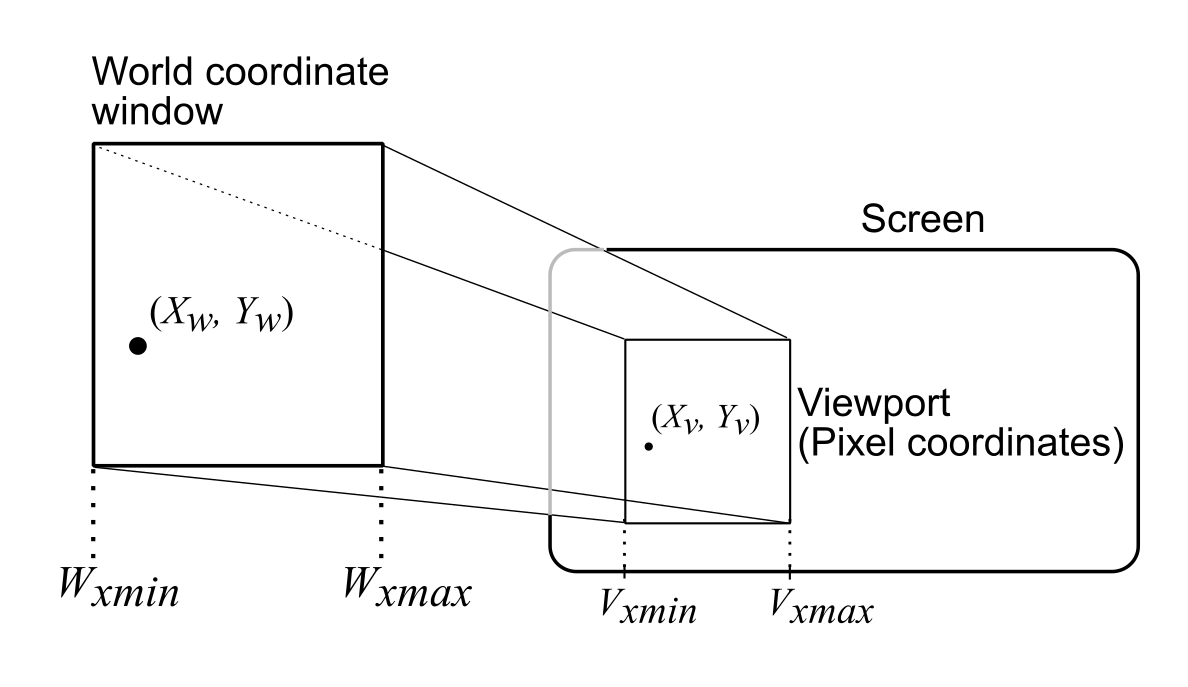
\includegraphics[scale=0.4]{normalisation}
  \centering
\end{figure}

We then perform normalisation to compute the pixel coordinates from the world coordinates, using simple ratios.
For the $x$ direction:
\[
  \frac{X_w - W_{xmin}}{W_{xmax} - W_{xmin}} = \frac{X_v - V_{xmin}}{V_{xmax} - V_{xmin}}
\]
\[
  X_v = \frac{(X_w - W_{xmin})(V_{xmax} - V_{xmin})}{W_{xmax} - W_{xmin}} + V_{xmin}
\]

With a similar expression for $y$.

From the known values, we can form a simple pair of linear equations:
\begin{align*}
  X_v &= AX_w + B \\
  Y_v &= CY_w + D
\end{align*}

If the window is moved or resized, we must re-calculate the constants $A, B, C, D$.

\subsection{Representing Planar Polygons}
Most graphical scenes and objects are built out of planar polyhedra, three-dimensional objects whose faces are all planar polygons (\textbf{faces} or \textbf{facets}).
To describe objects made of polygons, we need the \textbf{locations} of the vertices and their \textbf{topology}.

\begin{itemize}
  \item Numerical Data - 3D coordinates of vertices.
  \item Topological Data - what is connected to what.
\end{itemize}

\begin{figure}[h]
  \caption{Data for a polygon.}
  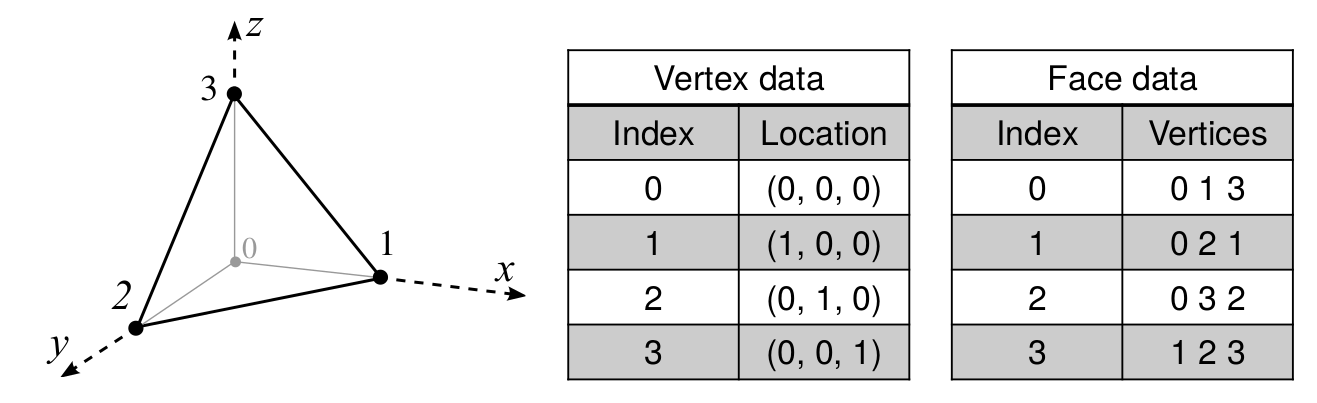
\includegraphics[scale=0.3]{polygon}
  \centering
\end{figure}

\subsection{Projections of Wire-Frame Models}
A \textbf{projection} transforms an $n$-dimensional space into an $m$-dimensional space, where $m < n$.
When projecting an object onto a surface, we first select a viewpoint then define \textit{projectors} or lines which join each vertex of the object to the viewpoint.
Where the projector intersects with the surface is defined as the projection of the corresponding vertex in the object.

The most common projections for viewing 3D scenes use a plane for the projection surface and straight lines for the projectors, these are \textbf{planar geometric projections}.
\textbf{Wire frame} models simply include points and lines, to render such a representation we need to specify only which edges join which points.
Other forms of rendering need to define the object faces.

There are two commons types of planar geometric projection:
\begin{itemize}
  \item \textbf{Parallel projection} - parallel projectors.
  \item \textbf{Perspective projection} - projectors pass through a single point (\textit{viewpoint}).
\end{itemize}

We first make some assumptions:
\begin{itemize}
  \item The viewpoint is at $z = - \infty$.
  \item The plane of projection is $z = 0$ (we can use coordinate transformations in 3D to make it so).
\end{itemize}

\subsection{Orthographic Projections}
In parallel projection, all projectors have the same direction $d$, and the viewpoint is considered to be at infinity.
For a vertex $V = (V_x, V_y, V_z)^\intercal$:
\[
  P = V + \mu d
\]

A special case is \textbf{orthographic projection}, where the projectors are perpendicular to the projection plane.
This means:
\[
  d = 
  \begin{pmatrix}
    0 \\
    0 \\
    -1
  \end{pmatrix}
\]

\begin{figure}[h]
  \caption{Parallel projection.}
  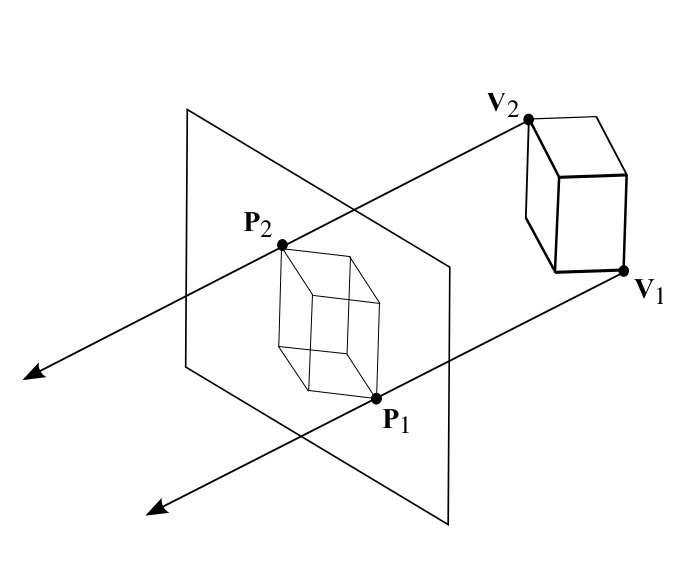
\includegraphics[scale=0.3]{parallel}
  \centering
\end{figure}

Which gives the Cartesian equations for each component:
\begin{align*}
  P_x &= V_x  & P_y &= V_y & P_z &= V_z - \mu
\end{align*}
Note that since $z = 0$, then $P_z = 0$.

This means we simply take the $x$ and $y$ coordinates:
\[
  P =
  \begin{pmatrix}
    V_x \\
    V_y \\
    0
  \end{pmatrix}
\]

\subsection{Perspective Projections}
Orthographic projections are fine in cases where we do not care about depth.
In \textbf{perspective projection}, all the projectors pass through one point in space, the \textit{centre of projection}.
If the centre of projection is on the opposite side of the plane of projection compared to the 3D object, the orientation of the image is the same as the object.
Otherwise if thecentre is between the plane and the object, the image is inverted.

\begin{figure}[h]
  \caption{Perspective projection where the viewpoint is on the opposite side of the object.}
  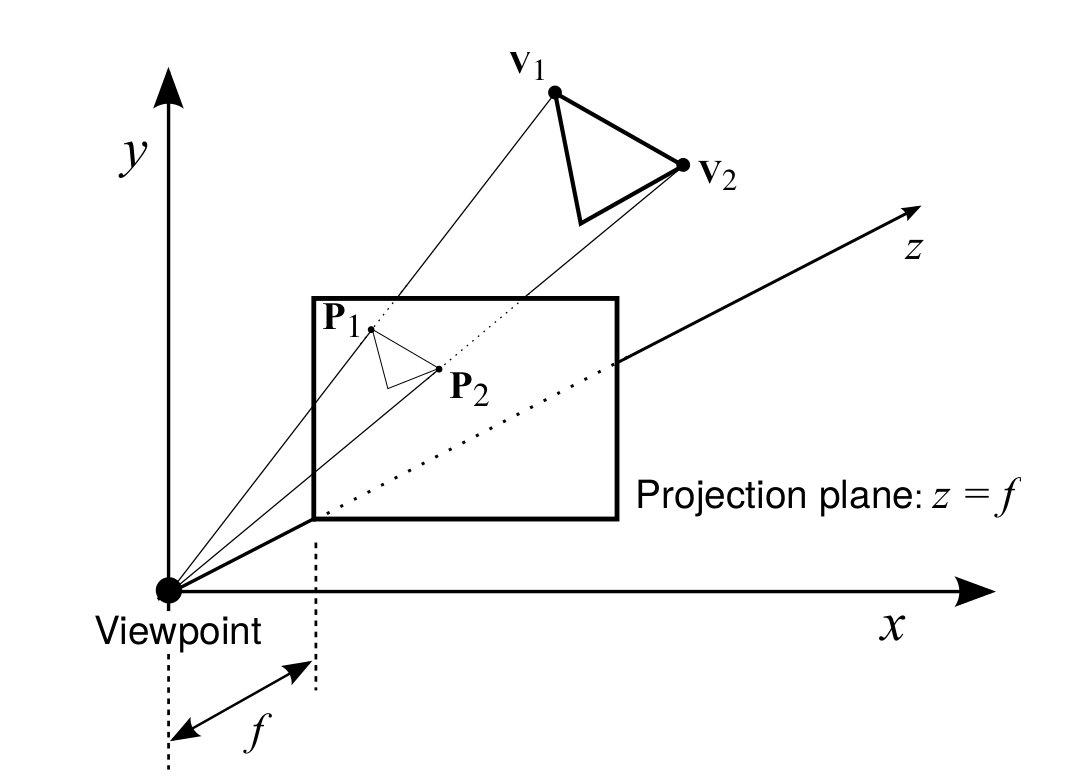
\includegraphics[scale=0.3]{perspective}
  \centering
\end{figure}

We first make two assumptions:
\begin{itemize}
  \item The centre of projection is at the origin.
  \item The projection plane is placed at a constant $z$ value, $z = f$.
\end{itemize}

The perspective projector equation from vertex $V$ is:
\[
  P = \mu V
\]

It follows that since $z = f$, then $f = \mu V_z$, and $\mu_p = f / V_z$.

This means:
\begin{align*}
  P_x = \mu_p V_x = \frac{fV_x}{V_z} && P_y = \mu_p V_y = \frac{fV_y}{V_z}
\end{align*}

We call $\mu_p$ the \textit{foreshortening} factor, if the object moves further away then $V_z$ increases and the image becomes smaller.

\subsection{Space Transformations}
Graphics scenes are defined in a particular coordinate system but we want to be able to view it at any point of our choosing.

We may also want to transform for other purposes:
\begin{itemize}
  \item Animating objects.
  \item Multiple instances.
  \item Reflections and other special effects.
\end{itemize}

In order to still be able to use canonical projection, we need to transform the coordinates of the scene so that the view direction is along the $z$-axis and the viewpoint at the origin.
That is, we want to change the coordinates of every point in the scene such that some chosen viewpoint $C$ becomes the origin, and the chosen view direction $d$ becomes the $z$-axis.
Transformation matricies can be used for nearly all simple transformations, except for translation using normal Cartesian coordinates.
We thus introduce \textbf{homogeneous coordinates}.

\subsubsection{Homogeneous Coordinates}
To express a point in homogeneous coordinates, we introduce a fourth coordinate (or \textit{ordinate}):
\[
  P =
  \begin{pmatrix}
    p_x \\
    p_y \\
    p_z \\
    s
  \end{pmatrix}
\]

The fourth ordinate is a scale factor, we use it to convert back to Cartesian form by dividing it into the other ordinates.
\[
  (p_x, p_y, p_z, s) \Leftrightarrow (\frac{p_x}{s}, \frac{p_y}{s}, \frac{p_z}{s})
\]
In most cases $s$ is $1$.

\subsubsection{Translation}
To represent translation:
\[
  \begin{pmatrix}
    1 & 0 & 0 & t_x \\
    0 & 1 & 0 & t_y \\
    0 & 0 & 1 & t_z \\
    0 & 0 & 0 & 1
  \end{pmatrix}
  \begin{pmatrix}
    p_x \\
    p_y \\
    p_z \\
    1
  \end{pmatrix}
  =
  \begin{pmatrix}
    p_x + t_x \\
    p_y + t_y \\
    p_z + t_z \\
    1
  \end{pmatrix}
\]

The inverse is:
\[
  \begin{pmatrix}
    1 & 0 & 0 & -t_x \\
    0 & 1 & 0 & -t_y \\
    0 & 0 & 1 & -t_z \\
    0 & 0 & 0 & 1
  \end{pmatrix}
\]

\subsubsection{Scaling}
To represent scaling:
\[
  \begin{pmatrix}
    s_x & 0 & 0 & 0 \\
    0 & s_y & 0 & 0 \\
    0 & 0 & s_z & 0 \\
    0 & 0 & 0 & 1
  \end{pmatrix}
  \begin{pmatrix}
    p_x \\
    p_y \\
    p_z \\
    1
  \end{pmatrix}
  =
  \begin{pmatrix}
    s_xp_x \\
    s_yp_y \\
    s_zp_z \\
    1
  \end{pmatrix}
\]

The inverse is:
\[
  \begin{pmatrix}
    1/s_x & 0 & 0 & 0 \\
    0 & 1/s_y & 0 & 0 \\
    0 & 0 & 1/s_z & 0 \\
    0 & 0 & 0 & 1
  \end{pmatrix}
\]


\subsubsection{Combining Transformations}
To combine transformations, we can multiply out their matrices and apply the transformation with the resultant matrix.

\begin{figure}[h]
  \caption{Importance of the order of transformations.}
  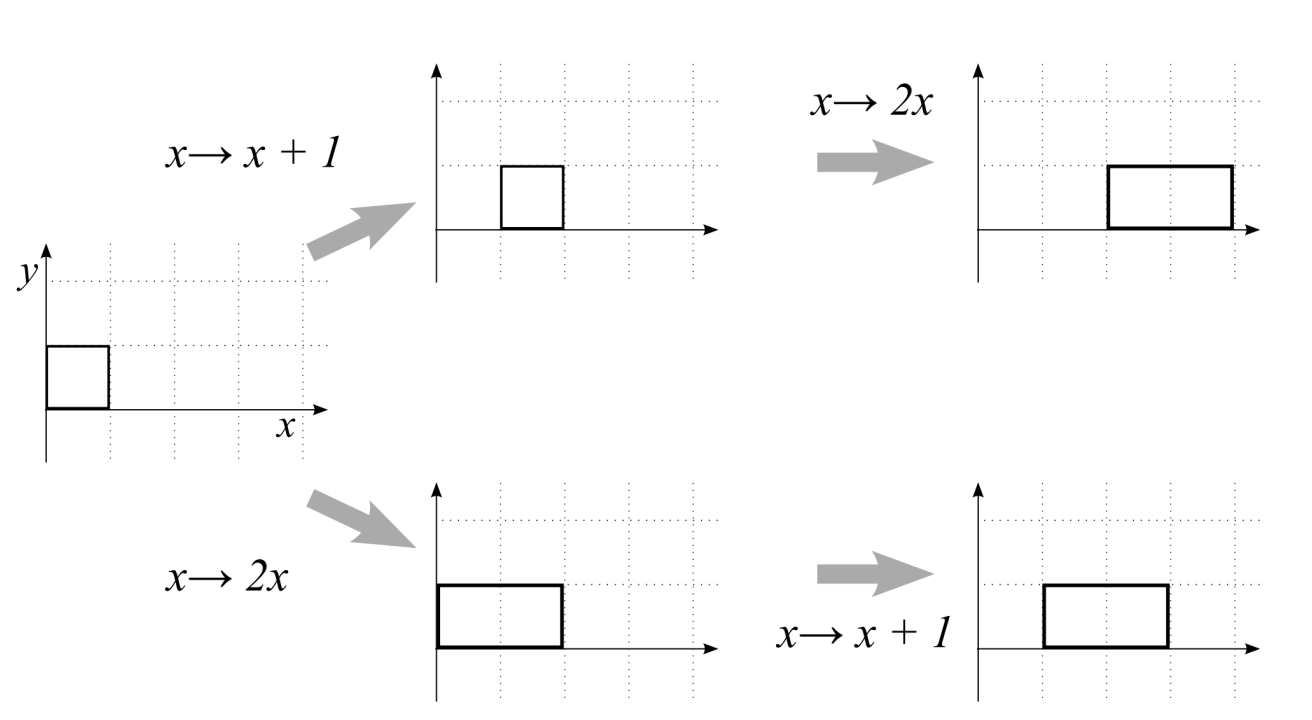
\includegraphics[scale=0.2]{combining}
  \centering
\end{figure}

Transformations are not necessarily commutative, it is important that they are carried out in the correct order.

\subsubsection{Rotation}
To define rotation we need an axis and an angle.
Matrices for rotation around the three cartesian axes are:
\begin{align*}
  \mathcal{R}_x &=
  \begin{pmatrix}
    1 & 0 & 0 & 0 \\
    0 & \cos \theta & -\sin \theta & 0 \\
    0 & \sin \theta & \cos \theta & 0 \\
    0 & 0 & 0 & 1
  \end{pmatrix} \\
  \mathcal{R}_y &=
  \begin{pmatrix}
    \cos \theta & 0 & \sin \theta & 0 \\
    0 & 1 & 0 & 0 \\
    -\sin \theta & 0 & \cos \theta & 0 \\
    0 & 0 & 0 & 1
  \end{pmatrix} \\
  \mathcal{R}_z &=
  \begin{pmatrix}
    \cos \theta &  -\sin \theta & 0 & 0 \\
    \sin \theta & \cos \theta & 0 & 0 \\
    0 & 0 & 1 & 0 \\
    0 & 0 & 0 & 1
  \end{pmatrix}
\end{align*}

\begin{figure}[h]
  \caption{Rotation of a coordinate ($z$-axis goes into the page).}
  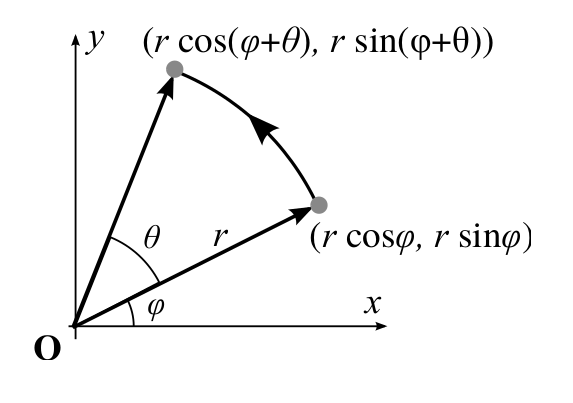
\includegraphics[scale=0.3]{deriverotate}
  \centering
\end{figure}

An example for how we derive $\mathcal{R}_z$ is as follows:
\[
  \begin{pmatrix}
    x \\
    y
  \end{pmatrix}
  =
  \begin{pmatrix}
    r \cos \varphi \\
    r \sin \varphi
  \end{pmatrix}
\]
\begin{align*}
  \begin{pmatrix}
    r \cos (\varphi + \theta) \\
    r \sin (\varphi + \theta)
  \end{pmatrix}
  &=
  \begin{pmatrix}
    r \cos \varphi \cos \theta - r \sin \varphi \sin \theta \\
    r \cos \varphi \sin \theta + r \sin \varphi \cos \theta
  \end{pmatrix} \\
  &=
  \begin{pmatrix}
    x \cos \theta - y \sin \theta \\
    x \sin \theta + y \cos \theta
  \end{pmatrix} \\
  &=
  \begin{pmatrix}
    \cos \theta & - \sin \theta \\
    \sin \theta & \cos \theta
  \end{pmatrix}
  \begin{pmatrix}
    x \\
    y
  \end{pmatrix}
\end{align*}

The $2 \times 2$ matrix is the same as the upper left corner of the matrix $\mathcal{R}_z$.

This assumes a left had axis system.
\begin{itemize}
  \item Rotation is \textbf{anti-clockwise} when looking along the axis of rotation.
  \item Rotation is \textbf{clockwise} when looking back towards the origin from the positive side of the axis.
\end{itemize}

To invert rotation, we rotate through an angle of $- \theta$, and note the follow relations:
\begin{align*}
  \cos(-\theta) &= \cos(\theta) & \sin(-\theta)=-\sin(\theta)
\end{align*}

Then for example:
\[
  \mathcal{R}_z(-\theta) = 
  \begin{pmatrix}
    \cos \theta & \sin \theta & 0 & 0 \\
    - \sin \theta & \cos \theta & 0 & 0 \\
    0 & 0 & 1 & 0 \\
    0 & 0 & 0 & 1
  \end{pmatrix}
\]

\section{Transformations for Animation}
In a viewer-centred application, we wish to view the scene from a moving position.
When the viewpoint changes, we need to transform all the coordinates of the scene.

\subsection{Flying Sequences}
Each moved viewpoint is a change of origin:
\begin{itemize}
  \item Let the required viewpoint be $C = (C_x, C_y, C_z)$.
  \item Let the required direction be $d = \begin{pmatrix} d_x \\ d_y \\ d_z \end{pmatrix}$.
\end{itemize}

The required transformation is split into three parts:
\begin{enumerate}
  \item Translation of the origin.
  \item Rotation about the $y$-axis.
  \item Rotation about the $x$-axis.
\end{enumerate}

\subsubsection{Translation of the Origin}

\begin{figure}[h]
  \caption{Translation of the origin.}
  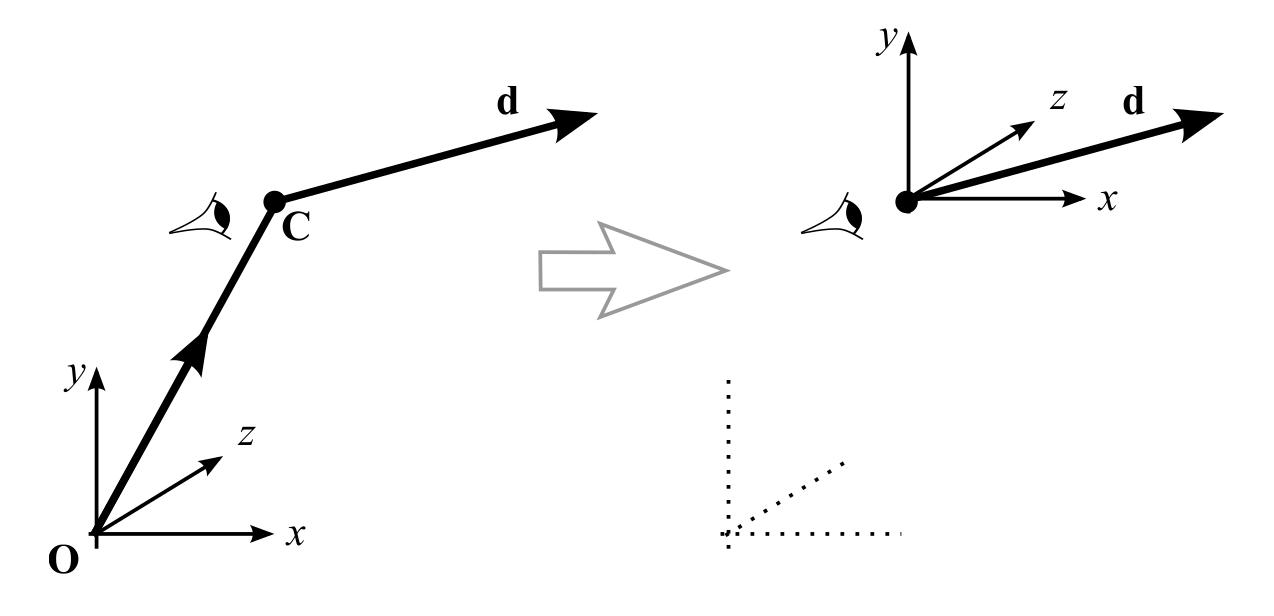
\includegraphics[scale=0.2]{transorigin}
  \centering
\end{figure}

We apply the transformation matrix:
\[
  \mathcal{A} =
  \begin{pmatrix}
    1 & 0 & 0 & -C_x \\
    0 & 1 & 0 & -C_y \\
    0 & 0 & 1 & -C_z \\
    0 & 0 & 0 & 1
  \end{pmatrix}
\]

\subsubsection{Rotation about the $y$-axis}
\begin{figure}[h]
  \caption{Rotation about the $y$-axis.}
  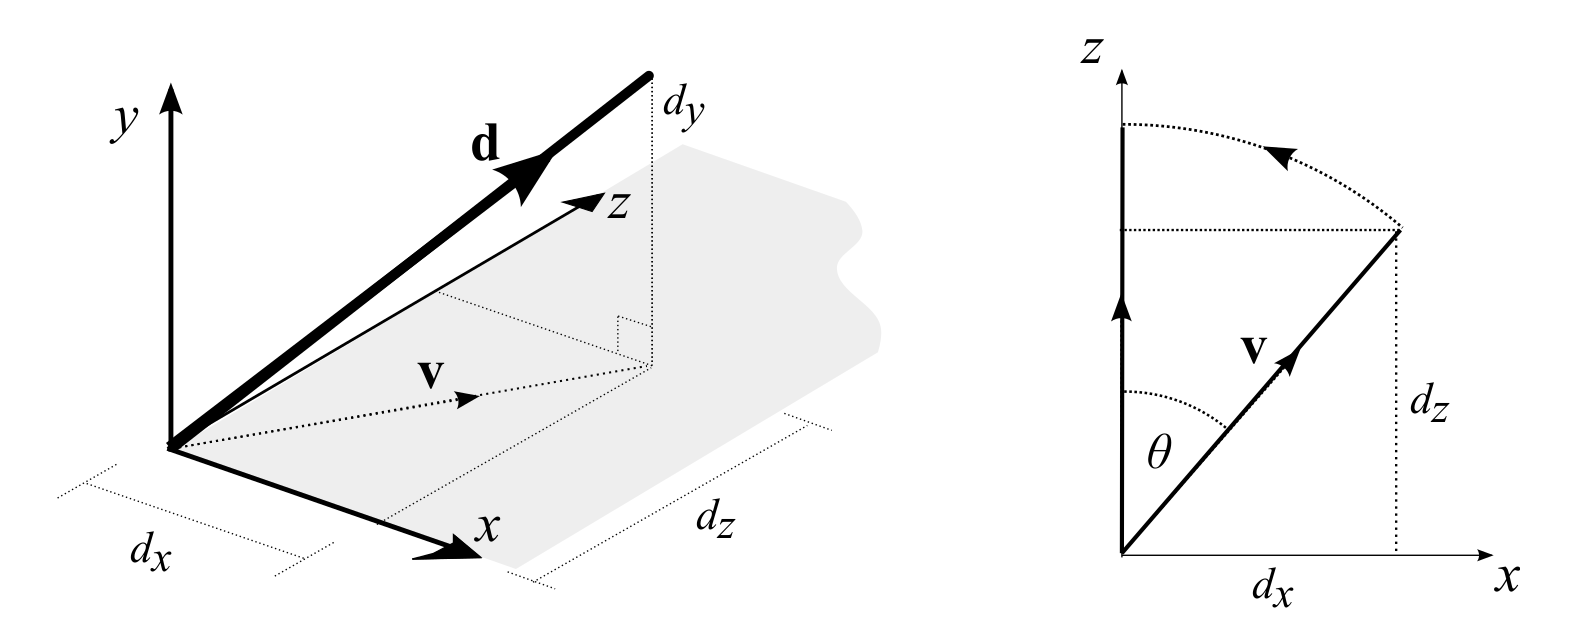
\includegraphics[scale=0.2]{roty}
  \centering
\end{figure}

We rotate about $y$ until $d$ is in the $y-z$ plane ($x = 0$):
\begin{align*}
  \lVert \textbf{v} \lVert = v = \sqrt{d_x^2 + d_z^2} && \cos \theta = d_z / v && \sin \theta = d_x / v
\end{align*}

\[
  \mathcal{B} =
  \begin{pmatrix}
    \cos \theta & 0 & -\sin \theta & 0 \\
    0 & 1 & 0 & 0 \\
    \sin \theta & 0 & \cos \theta & 0 \\
    0 & 0 & 0 & 1
  \end{pmatrix}
  =
  \begin{pmatrix}
    d_z / v & 0 & -d_x / v & 0 \\
    0 & 1 & 0 & 0 \\
    d_x / v & 0 & d_z / v & 0 \\
    0 & 0 & 0 & 1
  \end{pmatrix}
\]

\subsubsection{Rotation about the $x$-axis}
\begin{figure}[h]
  \caption{Rotation about the $x$-axis.}
  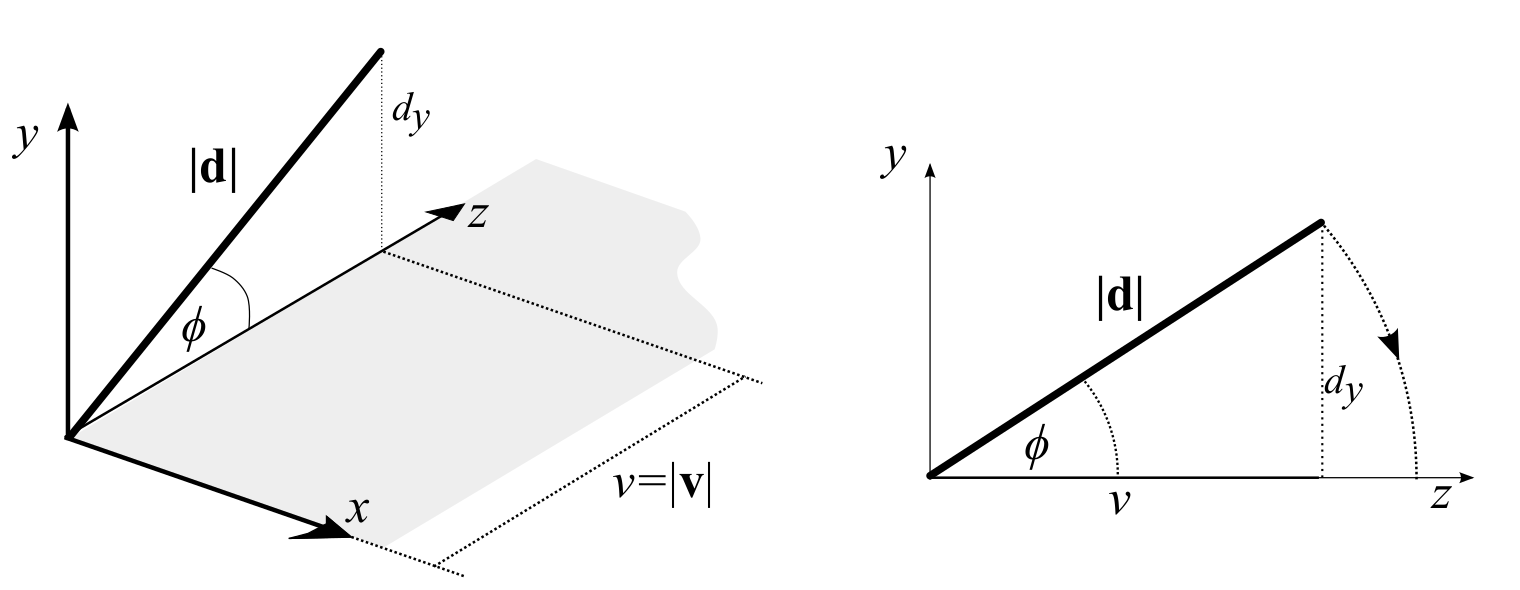
\includegraphics[scale=0.2]{rotx}
  \centering
\end{figure}

We then rotate about $x$ until $d$ points along the $z$-axis:
\begin{align*}
  v = \sqrt{d_x^2 + d_z^2} && \cos \phi = v / \lvert d \rvert && \sin \phi = d_y / \lvert d \rvert
\end{align*}

\[
  \mathcal{C} =
  \begin{pmatrix}
    1 & 0 & 0 & 0 \\
    0 & \cos \phi & -\sin \phi & 0 \\
    0 & \sin \phi & \cos \phi & 0 \\
    0 & 0 & 0 & 1
  \end{pmatrix}
  =
  \begin{pmatrix}
    1 & 0 & 0 & 0 \\
    0 & v / \lvert d \rvert & -d_y / \lvert d \rvert & 0 \\
    0 & d_y / \lvert d \rvert & v / \lvert d \rvert & 0 \\
    0 & 0 & 0 & 1
  \end{pmatrix}
\]

\subsubsection{Combining the Matrices}
\[
  \mathcal{T} = \mathcal{CBA}  
\]
Then for every point $\textbf{P}$ in the scene, we calculate:
\[
  \textbf{P}_t = \mathcal{T}\textbf{P}  
\]
The view is now in canonical form, and we can apply the standard perspective or othographic projection.

\subsubsection{Verticals}
\begin{figure}[h]
  \caption{Order of rotation affecting inversion.}
  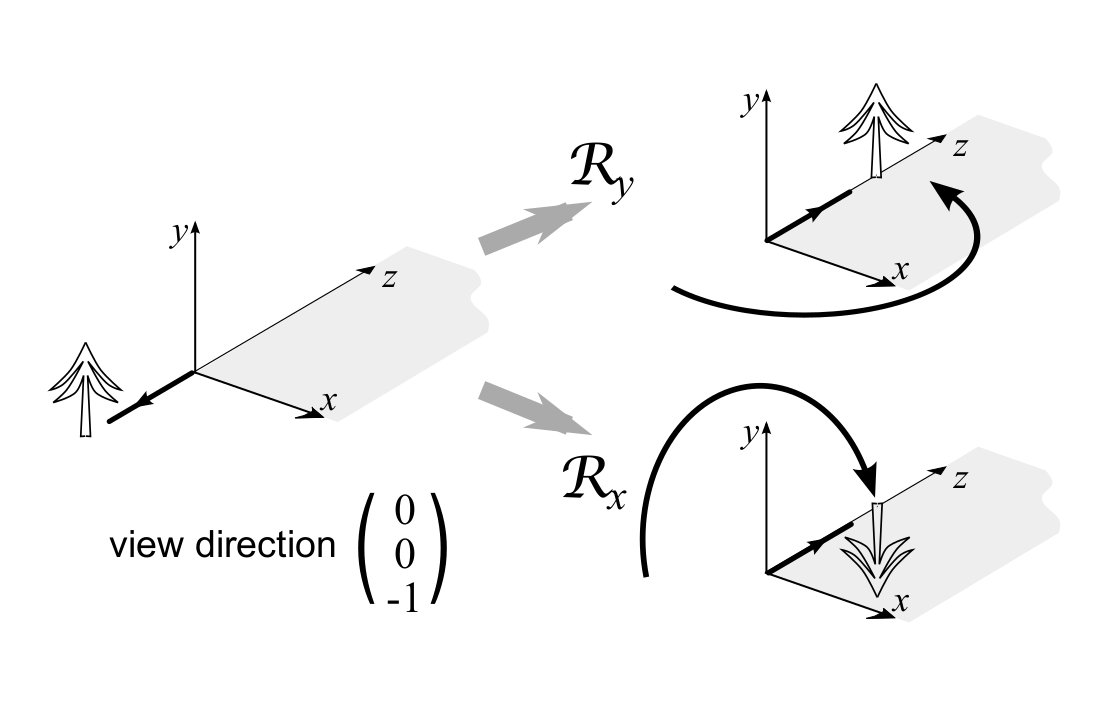
\includegraphics[scale=0.2]{invert}
  \centering
\end{figure}

Usually the $y$ direction is treated as vertical, by doing the $R_y$ transformation first, things will work out correctly.

However if we do the $R_x$ first, we could end up inverting the vertical.

\subsection{Rotation about a General Line}
To perform this transformation, we:
\begin{enumerate}
  \item Make the line of rotation one of the Cartesian axes.
  \item Rotate about the chosen axis.
  \item \textbf{Restore} the line to its original place.
\end{enumerate}

We achieve the first part through the same method as for \textit{flying sequences}: $\mathcal{CBA}$.

We then rotate about the $z$-axis, which is aligned with the general line.

Finally, we invert the initial matrices.

\[
  \mathcal{T} = \mathcal{A}^{-1} \mathcal{B}^{-1} \mathcal{C}^{-1} \mathcal{R}_z \mathcal{CBA}  
\]

\subsubsection{Other Effects}
Similar effects can be created using this approach.
\begin{eg}
  To make an object shrink (and stay in place):
  \begin{enumerate}
    \item Move the object to the origin.
    \item Apply a scaling matrix.
    \item Restore (move) the object to its place.
  \end{enumerate}
\end{eg}

\subsection{Projection by Matrix Multiplication}
\subsection{Orthographic Projection Matrix}
\[
  \mathcal{M}_o =
  \begin{pmatrix}
    1 & 0 & 0 & 0 \\
    0 & 1 & 0 & 0 \\
    0 & 0 & 0 & 0 \\
    0 & 0 & 0 & 1
  \end{pmatrix}
\]
\[
  \mathcal{M}_o
  \begin{pmatrix}
    x \\ y \\ z \\ 1
  \end{pmatrix}
  =
  \begin{pmatrix}
    x \\ y \\ 0 \\ 1
  \end{pmatrix}
\]

\subsection{Perspective Projection Matrix}
\[
  \mathcal{M}_p =
  \begin{pmatrix}
    1 & 0 & 0 & 0 \\
    0 & 1 & 0 & 0 \\
    0 & 0 & 0 & 0 \\
    0 & 0 & 1 / f & 0
  \end{pmatrix}
\]
\[
  \mathcal{M}_p
  \begin{pmatrix}
    x \\ y \\ z \\ 1
  \end{pmatrix}
  =
  \begin{pmatrix}
    x \\ y \\ z \\ z / f
  \end{pmatrix}
\]

We then normalise the result to get:
\[
  \begin{pmatrix} xf/z \\ yf/z \\ f \\ 1 \end{pmatrix}  
\]
as required.

\subsection{Singular}
Both projection matricies are singular, notice each has a column of zeroes.
This means they cannot be inverted: we cannot reconstruct the original 3D scene from a 2D image.

\subsection{Homogeneous Coordinates and Vectors}
\begin{itemize}
  \item \textbf{Position vectors} - $\begin{pmatrix} x \\ y \\ z \\ s \end{pmatrix}$.
    \begin{itemize}
      \item Non-zero final ordinate ($s$).
      \item Can be normalised into Cartesian form.
      \item \textit{Fixed point in space.}
    \end{itemize}
  \item \textbf{Direction vectors} - $\begin{pmatrix} x \\ y \\ z \\ 0 \end{pmatrix}$.
    \begin{itemize}
      \item Zero final ordinate.
      \item Have direction and magnitude.
      \item \textit{Not associated with a particular point.}
    \end{itemize}
\end{itemize}

\subsubsection{Addition of Vectors}
Adding \textbf{two direction vectors} results in a direction vector (notice the zero final ordinate):
\[
  \begin{pmatrix} x_i \\ y_i \\ z_i \\ 0 \end{pmatrix} 
  +
  \begin{pmatrix} x_j \\ y_j \\ z_j \\ 0 \end{pmatrix} 
  =
  \begin{pmatrix} x_i + x_j \\ y_i + y_j \\ z_i + z_j \\ 0 \end{pmatrix} 
\]

Adding a \textbf{direction vector to a position vector} results in a position vector:
\[
  \begin{pmatrix} X \\ Y \\ Z \\ 1 \end{pmatrix} 
  +
  \begin{pmatrix} x \\ y \\ z \\ 0 \end{pmatrix} 
  =
  \begin{pmatrix} X + x \\ Y + y \\ Z + z \\ 1 \end{pmatrix} 
\]

Adding \textbf{two position vectors} results in their mid-point:
\[
  \begin{pmatrix} X_a \\ Y_a \\ Z_a \\ 1 \end{pmatrix} 
  +
  \begin{pmatrix} X_b \\ Y_b \\ Z_b \\ 1 \end{pmatrix} 
  =
  \begin{pmatrix} X_a + X_b \\ Y_a + Y_b \\ Z_a + Z_b \\ 2 \end{pmatrix} 
  =
  \begin{pmatrix} (X_a + X_b) / 2 \\ (Y_a + Y_b) / 2 \\ (Z_a + Z_b) / 2 \\ 1 \end{pmatrix} 
\]

\subsection{Transformation Matrices}
\subsubsection{Structure}
\[
  \begin{pmatrix}
    q_x & r_x & s_x & C_x \\
    q_y & r_y & s_y & C_y \\
    q_z & r_z & s_z & C_z \\
    0 & 0 & 0 & 1
  \end{pmatrix}
\]
\begin{itemize}
  \item The bottom row is always $\begin{matrix}0&0&0&1\end{matrix}$.
  \item The columns comprise of three direction vectors and one position vector.
\end{itemize}

\subsubsection{Characteristics}
When we multiply a direction vector, the last ordinate ensures it is not affected by translation:
\[
  \begin{pmatrix}
    q_x & r_x & s_x & C_x \\
    q_y & r_y & s_y & C_y \\
    q_z & r_z & s_z & C_z \\
    0 & 0 & 0 & 1
  \end{pmatrix}
  \begin{pmatrix} * \\ * \\ * \\ 0 \end{pmatrix}
  =
  \begin{pmatrix} * \\ * \\ * \\ 0 \end{pmatrix}
\]

When we multiply a position vector, the last ordinate ensures all vectors have the same displacement:
\[
  \begin{pmatrix}
    q_x & r_x & s_x & C_x \\
    q_y & r_y & s_y & C_y \\
    q_z & r_z & s_z & C_z \\
    0 & 0 & 0 & 1
  \end{pmatrix}
  \begin{pmatrix} * \\ * \\ * \\ 1 \end{pmatrix}
  =
  \begin{pmatrix} * + C_x \\ * + C_y \\ * + C_z \\ 1 \end{pmatrix}
\]

If we do not shear the object, $q$, $r$, $s$ will remain orthogonal:
\[
  q \cdot r = r \cdot s = q \cdot s = 0  
\]

\subsubsection{Meaning of the Individual Columns}
When we multiply the matrix by unit vectors, we get the individual columns of the matrix:
\[
  \begin{pmatrix}
    q_x & r_x & s_x & C_x \\
    q_y & r_y & s_y & C_y \\
    q_z & r_z & s_z & C_z \\
    0 & 0 & 0 & 1
  \end{pmatrix}
  \begin{pmatrix} 1 & 0 & 0 & 0 \end{pmatrix}
  =
  \begin{pmatrix} q_x & q_y & q_z & 0 \end{pmatrix}
\]

This means that the columns are the original axis system after transforming to the new coordinate system:
\begin{itemize}
  \item \textbf{q} is the transformed $x$-axis.
  \item \textbf{r} is the transformed $y$-axis.
  \item \textbf{s} is the transformed $z$-axis.
  \item \textbf{C} is the transformed origin.
\end{itemize}

\subsubsection{Effect of a Transformation Matrix}
\begin{figure}[h]
  \caption{Effect of a transformation matrix.}
  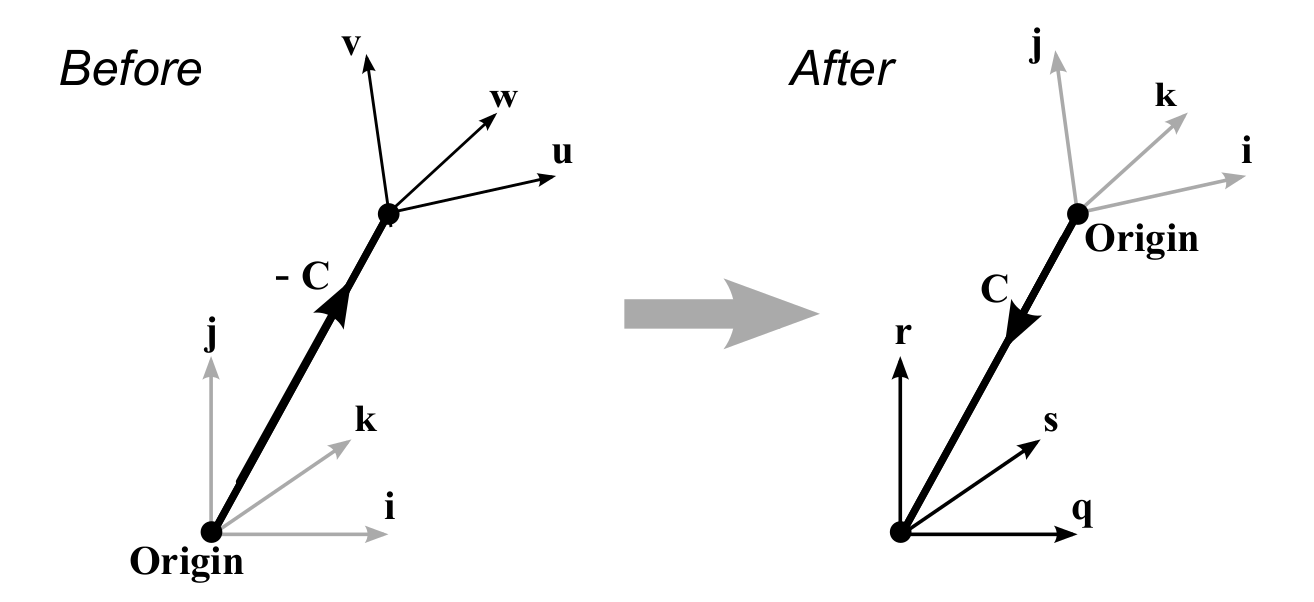
\includegraphics[scale=0.2]{effecttransform}
  \centering
\end{figure}

We get the old axes and origin in the new coordinate system:
\[
  \begin{pmatrix}
    q_x & r_x & s_x & C_x \\
    q_y & r_y & s_y & C_y \\
    q_z & r_z & s_z & C_z \\
    0 & 0 & 0 & 1
  \end{pmatrix}
  =
  \begin{bmatrix} \textbf{q} & \textbf{r} & \textbf{s} & \textbf{C} \end{bmatrix}
\]

\subsection{General Viewing Matrix Transformation}
Normally, we are not given the transformation matrix, but the view direction $\textbf{d}$ and location $\textbf{C}$ instead.

\subsubsection{Dot Product}
\begin{defn}
  The dot product is defined:
  \[
    P \cdot u = \lvert P \rvert \lvert u \rvert \cos \theta  
  \]
\end{defn}

\begin{figure}[h]
  \caption{The dot product as an ordinate of $P$.}
  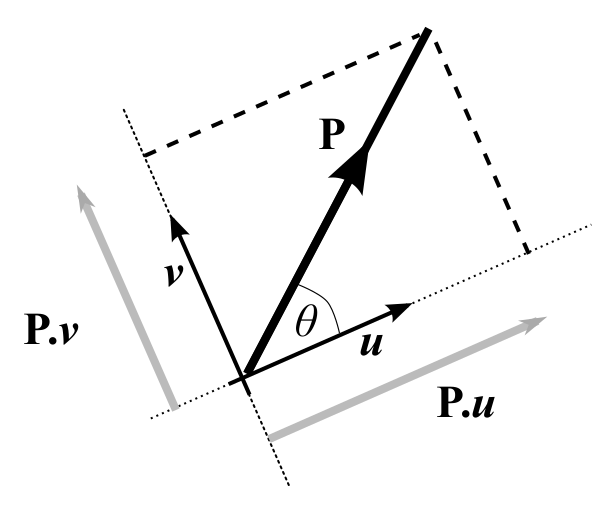
\includegraphics[scale=0.2]{dotproduct}
  \centering
\end{figure}

\begin{itemize}
  \item If $u$ is a unit vector, then $P \cdot u = \lvert P \rvert \cos \theta$.
  \item If $u$ is along a coordinate axis, then $P \cdot u$ is the ordinate of $P$ in the direction of $u$.
\end{itemize}

\subsubsection{Changing Axes by Projection}
\begin{figure}[h]
  \caption{Transforming a point $\textbf{P}$ to a different axes.}
  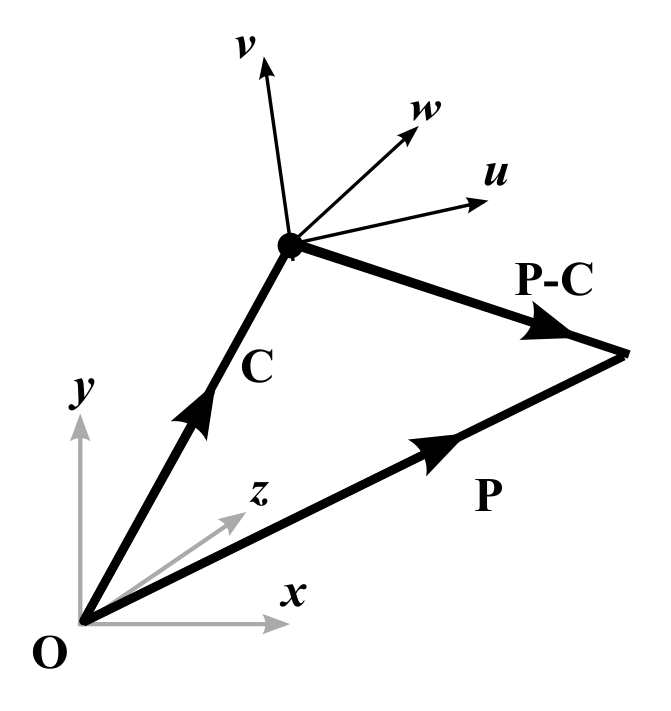
\includegraphics[scale=0.2]{changingaxes}
  \centering
\end{figure}

We can express projections using the dot product:
\begin{alignat*}{2}
  P_x^t &= (\textbf{P} - \textbf{C}) \cdot \textbf{u} &&= \textbf{P} \cdot \textbf{u} - \textbf{C} \cdot \textbf{u} \\
  P_y^t &= (\textbf{P} - \textbf{C}) \cdot \textbf{v} &&= \textbf{P} \cdot \textbf{v} - \textbf{C} \cdot \textbf{v} \\
  P_z^t &= (\textbf{P} - \textbf{C}) \cdot \textbf{w} &&= \textbf{P} \cdot \textbf{w} - \textbf{C} \cdot \textbf{w}
\end{alignat*}

In matrix notation:
\[
  \begin{pmatrix} P_x^t \\ P_y^t \\ P_z^t \\ 1 \end{pmatrix}
  =
  \begin{pmatrix}
    u_x & u_y & u_z & -\textbf{C} \cdot \textbf{u} \\ 
    v_x & v_y & v_z & -\textbf{C} \cdot \textbf{v} \\ 
    w_x & w_y & w_z & -\textbf{C} \cdot \textbf{w} \\ 
    0 & 0 & 0 & 1
  \end{pmatrix}
  \begin{pmatrix} P_x \\ P_y \\ P_z \\ 1 \end{pmatrix}
\]

By maintaining values of $\textbf{C}, \textbf{u}, \textbf{v}, \textbf{w}$ throughout an animation sequence, we can write down the correct scene transformation matrix.

\subsubsection{Returning to Flying Sequences}
As we know $\textbf{d}$ is the direction of the new axis, then
\[
  \textbf{w} = \frac{\textbf{d}}{\lvert \textbf{d} \rvert}
\]

We can write $\textbf{u}$ in terms of some vector $\textbf{p}$ in the horizontal direction:
\[
  \textbf{u} = \frac{\textbf{p}}{\lvert \textbf{p} \rvert}
\]
and set $p_y = 0$ to ensure it has no vertical component.

We can write $\textbf{v}$ in terms of some vector $\textbf{q}$ in the vertical direction:
\[
  \textbf{v} = \frac{\textbf{q}}{\lvert \textbf{q} \rvert}
\]
and force $q_y = 1$ to ensure it has a positive $y$ component.

We now have:
\begin{align*}
  \textbf{p} &= \begin{pmatrix} p_x \\ 0 \\ p_z \end{pmatrix}
  & \textbf{q} &= \begin{pmatrix} q_x \\ 1 \\ q_z \end{pmatrix}
\end{align*}

It must be that:
\[
  \textbf{d} = \textbf{p} \times \textbf{q} 
\]
since $\textbf{d}$ is orthogonal to both, and the magnitude of the new vectors has not been set.

Evaluating the cross products results in:
\begin{align*}
  d_x &= -p_z \\
  d_y &= p_zq_x - p_xq_z \\
  d_z &= p_x
\end{align*}

Which means:
\[
  \textbf{p} = \begin{pmatrix} d_z \\ 0 \\ -d_x \end{pmatrix} 
\]

Using the dot product with $\textbf{p}$ and $\textbf{q}$, then:
\[
  \textbf{p} \cdot \textbf{q} = p_xq_x + p_zq_z = 0
\]
which we solve with the result from the cross product:
\[
  d_y = p_zq_x - p_xq_z
\]

Once we have expressions for $\textbf{p}$ and $\textbf{q}$ in terms of given vector $\textbf{d}$, then we have obtained:
\begin{align*}
  \textbf{u} &= \frac{\textbf{p}}{\lvert \textbf{p} \rvert} &
  \textbf{v} &= \frac{\textbf{q}}{\lvert \textbf{q} \rvert} &
  \textbf{w} &= \frac{\textbf{d}}{\lvert \textbf{d} \rvert}
\end{align*}
which we use to write down:
\[
  \begin{pmatrix}
    u_x & u_y & u_z & -\textbf{C} \cdot \textbf{u} \\ 
    v_x & v_y & v_z & -\textbf{C} \cdot \textbf{v} \\ 
    w_x & w_y & w_z & -\textbf{C} \cdot \textbf{w} \\ 
    0 & 0 & 0 & 1
  \end{pmatrix}
\]


\end{document}
